

    \section{Número de oxidación}\label{subsec:numero-de-oxidacion}

    \begin{center}
        \begin{definicion}[width=0.9\textwidth]{Número de Oxidación}
            El \negrita{número de oxidación} es una carga eléctrica asignada a cada átomo (proviene de perder o ganar electrones).
        \end{definicion}
    \end{center}


    Podemos tener en cuenta las siguientes consideraciones para facilitar obtener el estado de oxidación:

    \begin{enumerate}[label=\numberballmDarkTeal]
        \item Es cero para todos los elementos en estado neutro.
        \item Para las especies iónicas monoatómicas coincide con la carga del ion. \ch{Al^{3+}} tiene un número de oxidación de \num{+3}, el del \ch{S^2-} es de \num{-2}.
        \item Para el hidrógeno en los hidruros metálicos es siempre \num{-1}.
        \item En los elementos del grupo 1 (alcalinos) es siempre \num{+1} y en los del grupo 2 (alcalinotérreos) es \num{+2}.
        \item En los halógenos (en compuestos binarios) es siempre \num{-1}.
        \item En las moléculas neutras, la suma de todos los números de oxidación es \num{0}.
        \item En los iones poliatómicos, la suma de todos los números de oxidación es igual a su carga neta.
    \end{enumerate}

    Siempre que en una reacción se produzcan cambios en los números de oxidación será una reacción redox.
    En la siguiente reacción de formación de \ch{CO2} vemos como el carbono pasa de \num{0} a \num{+4} mientras que el oxígeno pasa de \num{0} a \num{-2}.

    \begin{equation*}
        \ox{0,C} \ch{+} \ox{0,O2} \ch{->} \ox{+4,C}\ \ox{-2,O2}
    \end{equation*}

    En este otro ejemplo vemos como el manganeso pasa de \num{+7} a \num{+4} mientras que el yodo pasa de \num{-1} a \num{0}.

    \begin{equation*}
        \ox{1,K}\ \ox{7,Mn}\ \ox{-2,O4}\ \ch{+} \ox{1,K}\ \ox{-1,I}\ + \ox{1,H2}\ \ox{-2,O}\ \ch{->} \ox{0,I2} \ch{+} \ox{4,Mn}\ \ox{-2,O2} \ch{+} \ox{1,K}\ \ox{-2,O}\ \ox{1,H}
    \end{equation*}

    \subsection{Concepto de oxidación y reducción}\label{subsec:concepto-de-oxidacion-y-reduccion}

    Antiguamente, el concepto de oxidación se utilizaba para indicar que un compuesto aumentaba el número de átomos de oxígeno mientras que la reducción se utilizaba para indicar la pérdida de átomos de oxígeno.
    Estas definiciones no son aplicables a todos los procesos redox por lo que se tuvieron que redefinir los términos de reducción y oxidación de manera que pudieran ser aplicables a todos los casos.
    Actualmente, la oxidación y la reducción la podemos definir como:

    \caja{La \negrita{oxidación} es la pérdida de \el{} por lo que aumentará su número de oxidación.
        \begin{align*}
            \ch{M  & -> M+ + 1 \el}\separ
            \ch{Na & -> Na+ + 1 \el}\separ
            \ch{Ca & -> Ca^{2+} + 2 \el}
        \end{align*}
    }

    \caja{La \negrita{reducción} es la ganancia de \el{} por lo que disminuirá su número de oxidación.
        \begin{align*}
            \ch{X + 1 \el & -> X- }\separ
            \ch{S + 2 \el & -> S^{2-} }\separ
            \ch{F + 1 \el & -> F^- }
        \end{align*}
    }

    \subsection{Pares redox}\label{subsec:pares-redox}

    En las reacciones de \negrita{transferencia de electrones} se necesita una especie que se oxide y otra especie que se reduzca, por este motivo siempre hablamos de \negrita{pares redox}.

    En las reacciones redox debemos introducir dos nuevos conceptos:


    \caja{\negrita{Oxidante} es la especie que se reduce aceptando electrones a la otra especie.
        \begin{equation*}
            \text{Oxidante}_1 + {\color{myGreen} n\ \el} \ch{->[Reducción]} \text{Reductor}_1
        \end{equation*}
    }

    \caja{\negrita{Reductor} es la especie que se oxida cediendo electrones a la otra especie.
        \begin{equation*}
            \text{Reductor}_2  \ch{->[Oxidación]} \text{Oxidante}_2 \ch{+} {\color{myGreen} n\ \el}
        \end{equation*}
    }

    Por lo tanto, una reacción redox la podemos representar como:

    \begin{equation*}
        \text{Oxidante}_1 + \text{Reductor}_2  \ch{->} \text{Reductor}_1 + \text{Oxidante}_2
    \end{equation*}

    Si nos damos cuenta, el tratamiento es muy similar a las reacciones ácido-base pudiendo decir por tanto que tendremos \negrita{pares redox conjugados}.

    De manera general (similar a los ácidos y bases) podemos decir que:

    \begin{enumerate}[label=\(\bullet\)]
        \item Un reductor fuerte tendrá un oxidante conjugado débil y viceversa.
        \item Un oxidante fuerte tendrá un reductor débil y viceversa
    \end{enumerate}

    Al igual que en los ácidos y las bases, una especie actuará como oxidante o como reductor dependiendo de la naturaleza de la otra especie.

    \subsection{Separación de ácidos, bases y sales}\label{subsec:separacion-de-acido-bases-y-sales}

    Para el ajuste de reacciones químicas, es fundamental saber separar los iones en los ácidos y en las sales que intervienen en el proceso.
    A continuación se darán algunas reglas que nos permita separarlos de manera correcta pero antes debemos indentificar previamente lo que es un ácido, una base y un sal.

    \begin{enumerate}[label=\numberballmDarkTeal]
        \item \negsubro{Ácidos}.
        Para separar correctamente los ácidos debemos seguir las siguientes reglas:

        \begin{enumerate}[label=\letraminuscula]
            \item Solo podemos separar los hidrógenos del ácido.
            \item El oxígeno que está unido al átomo central, nunca se puede separar de ese átomo.
            \item El hidrógeno que separaremos siempre tendrá una carga positiva quedando siempre como \ch{H\pch[]}.
            \item El átomo central unido al oxígeno no se puede separar.
            \item El átomo central junto al oxígeno tendrán tantas cargas negativas como hidrógenos hayamos quitado.
            Por ejemplo, en el caso del \ch{H2SO4} tendremos: \ch{2 H\pch[]} y \ch{SO4\mch[2]}.
        \end{enumerate}
        \item \negsubro{Bases}
        Para separar correctamente las bases debemos seguir las siguientes reglas:
        \begin{enumerate}[label=\letraminuscula]
            \item En los hidróxidos se separa el metal del grupo hidroxilo, el grupo hidroxilo tendrá siempre carga negativa (\ch{OH-}) mientras que el metal tendrá tantas cargas positivas como número de grupos \ch{OH} tenga.
            \item Una base que no sea un hidróxido no se puede separar
        \end{enumerate}
        \item \negsubro{Sales}
        Para separar las sales debemos saber que:
        \begin{enumerate}[label=\letraminuscula]
            \item La especie de la derecha tendrá carga negativa.
            \item La especie de la izquierda tendrá carga positiva.
            \item En las oxosales debemos separar el metal (elemento de la izquierda) del átomo central junto al oxígeno. Para conocer su carga se siguen las mismas reglas que en los ácidos.
        \end{enumerate}
    \end{enumerate}

    \subsection{Ajuste de ecuaciones redox. Método del ion-electrón}\label{subsec:ajuste-de-ecuaciones-redox.-metodo-del-ion-electron}

    En las reacciones redox, ajustar una reacción por tanteo puede ser algo complejo y por este motivo, se utiliza el \negrita{método del ion-electrón}

    \subsubsection{Ajuste de reacciones redox en medio ácido}

    Consideremos la siguiente reacción:

    \begin{equation*}
        \ch{KI + KMnO4 + H2SO4 -> K2SO4 + MnSO4 + H2O + I2}
    \end{equation*}

    \begin{enumerate}[label=\numberballmDarkTeal]
        \item Escribimos los números de oxidación encima de cada símbolo atómico.
        \begin{equation*}
            \ox{1,K}\ \ \ox{-1,I}\ \ch{+} \ox{1,K}\ \ox{7,Mn}\ \ox{-2,O4}\ \ch{+} \ox{1,H2}\ \ox{6,S}\ \ox{-2,O4}\ \ch{->} \ox{1,K2}\ \ox{6,S}\ \ox{-2,O4}\ \ch{+} \ox{2,Mn}\ \ox{6,S}\ \ox{-2,O4}\ \ch{+} \ox{1,H2}\ \ox{-2,O}\ \ch{+} \ox{0,I2}
        \end{equation*}
        \item Detectar las especies que se reducen y se oxidan: Vemos que el \ch{Mn} se reduce pasando de \num{+7} a \num{+2} mientras que el yodo se oxida pasando de \num{-1} a \num{0}.
        \item Separamos los iones en las sales (esta opción puede omitirse).
        \begin{equation*}
            \ch{K+ + I- + K+ + MnO4- + 2 H+ + SO4^{2-} -> 2 K+ + SO4^{2-} + Mn^{2+} + SO4^{2-} + H2O + I2}
        \end{equation*}
        \item Escribimos las semirreacciones de oxidación y reducción:
        \begin{equation*}
            \text{Semirreacción. Oxidación:}\qquad \ch{I- -> I2}
        \end{equation*}
        \begin{equation*}
            \text{Semirreacción. Reducción:}\qquad \ch{MnO4- -> Mn\pch[2]}
        \end{equation*}
        \item Se ajustan las semirreacciones.
        Si en algún término falta oxígeno, se añade en forma de moléculas de \water.
        Si necesitamos añadir \ch{H}, se hace directamente como \ch{H+}.
        Una vez terminado, igualamos eléctricamente la reacción sumando o restando electrones que hagan falta.
        \item
        \begin{gather*}
            \text{Ox:}\qquad \ch{2 I- -> I2 + 2 \el} \separ
            \text{ó}\separ
            \text{Ox:}\qquad \ch{2 I- ->[{\color{red} \(-\) 2 \el}] I2}
        \end{gather*}

        Para la otra reacción de reducción tendremos que:

        \begin{equation*}
            \text{Red:}\qquad \ch{MnO4- + 8 H+ ->[{\color{blue}\(+ 5\ \el\)}] Mn^{2+} + 4 \water }
        \end{equation*}

        \item Ahora multiplicamos una o ambas semirreacciones por el número de electrones ganados o perdidos en la otra reacción.
        Si podemos simplificar los números, lo hacemos.

        A continuación sumamos ambas ecuaciones.
        \begin{equation*}
            \begin{aligned}
                5 \times \biggl( \ch{2 I-}        & \ch{->[{\color{red} \(-\) 2 \el}]} \ch{I2} \biggr)\separ
                2 \times \biggl(\ch{MnO4- + 8 H+} & \ch{->[{\color{blue}\(+ 5\ \el\)}]} \ch{Mn^{2+} + 4 \water }\biggr)\separ
                \midrule
                \ch{10 I- + 2 MnO4- + 16 H+       & -> 5 I2 + 2 Mn^{2+} + 8 \water}                                           \\
            \end{aligned}
        \end{equation*}
        La ecuación obtenida se denomina \negrita{ecuación iónica}
        \item Simplificamos el número de moléculas de agua y el número de \ch{H+}.
        En este caso no es necesario.
        \item Ahora trasladamos los coeficiente estequiométricos de la ecuación iónica a la ecuación global.
        % \azuln{Si una  especie química se ve afectada por dos posibles coeficientes, se escoge siempre el de mayor y los iones sobrantes se tienen en cuenta al otro lado de la reacción.}
        \begin{equation*}
            10\ {\color{red}\ch{K}}\ch{I} + \ch{2 KMnO4} + {\color{red}\ch{8 H2}}\ch{SO4} \ch{->} \ch{5 I2 + 2 MnSO4 + 8 \water}
        \end{equation*}
        \item Ahora realizamos un ajuste final por tanteo.
        \begin{equation*}
            10\ {\color{red}\ch{K}}\ch{I} + \ch{2 KMnO4} + {\color{red}\ch{8 H2}}\ch{SO4} \ch{->}{\color{blue}\ch{6 K2SO4}}\ch{+} \ch{5 I2 + 2 MnSO4 + 8 \water}
        \end{equation*}
        \item A esta última reacción se le conoce como \negrita{reacción molecular}
    \end{enumerate}

    \subsubsection{Medio básico}

    Llevaremos a cabo el ajuste de la reacción entre el clorato sódico y cloruro de cromo (III) en presencia de hidróxido de sodio para formar cromato de sodio, cloruro de sodio y agua.

    La reacción sin ajustar sería:

    \begin{equation*}
        \ch{CrCl3 + NaClO3 + NaOH -> Na2CrO4 + H2O + NaCl}
    \end{equation*}


    \begin{enumerate}[label=\numberballmDarkTeal]
        \item Escribimos los números de oxidación encima de cada símbolo atómico para detectar los cambios que se producen.
        \begin{equation*}
            \ox{3,Cr}\ \ox{-1,Cl3}\ \ch{+} \ox{1,Na}\ \ox{+5,Cl}\ \ox{-2,O3}\ \ch{+} \ox{1,Na}\ \ox{-2,O}\ \ox{1,H}\ \ch{->} \ox{1,Na2}\ \ox{6,Cr}\ \ox{-2,O4}\ \ch{+} \ox{1,H2}\ \ox{-2,O}\ \ch{+} \ox{1,Na}\ \ox{-1,Cl}
        \end{equation*}
        \item Detectar las especies que se reducen y se oxidan: Vemos que el \ch{Cl} se reduce pasando de \num{+5} a \num{-1} mientras que el \ch{Cr} se oxida pasando de \num{+3} a \num[retain-explicit-plus]{+6}.
        \item Separamos los iones de las sales (esta opción puede omitirse).
        \begin{equation*}
            \ch{Cr^{3+} + 3 Cl- + Na+ + ClO3- + Na + \Hyd -> 2 Na+ + CrO4^{2-} + H2O + Na+ + Cl-}
        \end{equation*}
        \item Escribimos las semirreacciones de oxidación y reducción:
        \begin{equation*}
            \text{Ox:}\qquad \ch{Cr^{3+} -> CrO4^{2-} }
        \end{equation*}
        \begin{equation*}
            \text{Red:}\qquad \ch{ClO3- -> Cl-}
        \end{equation*}
        \item Se ajustan las semirreacciones.
        Si en algún término falta \ch{O}, se añade en forma de moléculas de \water.
        Si necesitamos añadir \ch{H}, se hace directamente como \ch{H+}.
        Una vez terminado, igualamos eléctricamente la reacción sumando o restando electrones que hagan falta.
        \begin{gather*}
            \text{Ox:}\qquad \ch{Cr^{3+} + 4 \water->[{\color{red}\num{-3}\ \el}] CrO4^{2-} + 8 H+}
        \end{gather*}
        Para la otra reacción de reducción tendremos que:
        \begin{equation*}
            \text{Red:}\qquad \ch{ClO3- + 6 H+ ->[{\color{blue}\num{+6}\ \el }] Cl- + 3 \water }
        \end{equation*}
        \item Ahora multiplicamos una o ambas semirreacciones por el número de electrones ganados o perdidos en la otra reacción.
        Si podemos simplificar los números, lo hacemos.
        Finalmente sumamos ambas ecuaciones.

        \begin{equation*}
            \begin{aligned}
            {\color{blue}2\ \cancel{6}}
                \times \biggl( \ch{Cr^{3+} + 4 \water         & ->[{\color{red}\num{-3}\ \el}] CrO4^{2-} + 8 H+}\biggr)\separ
                {\color{red}1\ \cancel{3}} \times \biggl(\ch{ClO3- + 6 H+                 & ->[{\color{blue}\num{+6}\ \el }] Cl- + 3 \water }\biggr)\separ
                \midrule
                \ch{2 Cr^{3+} + \(\cancelto{5}{8}\) H2O + ClO3- + \(\cancelto{0}{6}\) H+ & -> 2 CrO4^{2-} + \(\cancelto{10}{16}\) H+ + Cl- + \(\cancelto{0}{3}\) H2O} \\
                \text{Simplificamos:}                                                                                                                                  \\
                \ch{2 Cr^{3+} + 5 H2O + ClO3-                                            & -> 2 CrO4^{2-} + 10 H+ + Cl- }
            \end{aligned}
        \end{equation*}

        \hdashrule{\textwidth}{1pt}{1pt}

        \begin{center}
            Hasta aquí todo igual que en el caso del medio ácido.
        \end{center}
        \hdashrule{\textwidth}{1pt}{1pt}

        \item Ahora, para conseguir el medio básico, lo que hacemos es añadir iones \Hyd\  tanto a la izquierda como a la derecha como número de iones \ch{H\pch} tengamos:
        \begin{reaction*}
            2 Cr^{3+} + 5 H2O + ClO3- + 10 OH- -> 2 CrO4^{2-} + 10 H+ + Cl- + 10 OH-
        \end{reaction*}
        Los grupos \Hyd y \ch{H+} formarán moléculas de \water\ quedando finalmente tras simplificar como:
        \begin{reaction}
            2 Cr\pch[3] + ClO3\mch{} + 10 OH- -> 2 CrO4\mch[2] + 5 H2O + Cl-  "\label{rxn:ionica_medio_basico}"
        \end{reaction}
        La reacción~\eqref{rxn:ionica_medio_basico} es la \negrita{reacción / ecuación iónica}
        \item Ahora trasladamos los coeficiente estequiométricos de la ecuación iónica a la ecuación global.
        % \azuln{Si una  especie químicas se ve afectada por dos posibles coeficientes, se escoge siempre el de mayor y los iones sobrantes se tienen en cuenta al otro lado de la reacción.}
        \begin{equation*}
            2\ {\color{red}\ch{Cr}}\ch{Cl3} + \ch{NaClO3} + {\color{red}\ch{10 NaOH}} \ch{->} \ch{2 Na2CrO4 + 5 H2O + 7 NaCl}
        \end{equation*}
        A esta última reacción se le conoce como \negrita{reacción molecular}
    \end{enumerate}


    \section{Valoraciones redox}\label{sec:valoraciones-redox}

    Del mismo modo que en las valoraciones ácido-base, podemos calcular la concentración de un reactivo oxidante o reductor a partir de su valoración con otro reactivo de concentración conocida.

    Sea la siguiente reacción general donde:
    \begin{equation*}
        \ch{a\ Oxidante1 + b\ Reductor2 -> m\ Reductor1 + n\ Oxidante2}
    \end{equation*}

    Al igual que en el caso ácido base, se tiene que cumplir que:
    \begin{equation}
        b\cdot V_{\text{Oxidante\subin{1}}}\cdot \conc{Oxidante1} = a\cdot V_{\text{Reductor\subin{2}}}\cdot \conc{Reductor2}\label{eq:volumentria_molaridad}
    \end{equation}

    En la ecuación \eqref{eq:volumentria_molaridad} la concentración de las especies se representa en molaridad.
    Si nos fijamos, se trata de un tratamiento muy similar al utilizado en las valoraciones ácido-base.

    Otra forma de llevar a cabo es haciendo uso de la normalidad y teniendo en cuenta que:
    \begin{equation*}
        n\text{º equivalente-gramo Oxidante\subin{1}} = n\text{º equivalente-gramo Reductor\subin{2}}
    \end{equation*}

    Si sabemos que:

    \begin{equation*}
        n\text{º equivalente-gramo} = N\cdot V
    \end{equation*}

    tendremos por tanto que:

    \begin{equation*}
        N_{\text{oxidante}}\cdot V_ {\text{oxidante}} = N_{\text{reductor}}\cdot V_ {\text{reductor}}
    \end{equation*}

    Sin embargo aunque esta última ecuación es muy útil, en la mayoría de las ocasiones las concentraciones se dan en molaridad.
    En este caso, esta última expresión la podemos transformar en:

    \begin{equation*}
        \text{Valencia oxidante}\ V_{\text{oxidante}} \ M_{\text{oxidante}} = \text{Valencia reductor}\ V_{\text{reductor}} \ M_{\text{reductor}}
    \end{equation*}

    En este caso, la valencia del oxidante o el reductor será el número de electrones ganados (si es el caso del oxidante) o el número de electrones perdidos (si es el reductor)

    Sea la siguiente ecuación:
    \begin{equation*}
        \ch{Fe + Ce\pch[4] -> Fe\pch[3] + Ce\pch[3]}
    \end{equation*}

    Vemos que en este caso el reductor es el \ch{Fe\pch[2]} puesto que es la especie que se oxida según la ecuación:
    \begin{equation*}
        \ch{Fe -> Fe\pch[3] + 3 \el}
    \end{equation*}

    Por lo tanto, el número de equivalente gramo del \ch{Fe}  será: \(3\cdot \text{moles de } \ch{Fe}\)


    \section{Tipos de reacciones Redox según su espontaneidad}\label{sec:tipos-de-reacciones-redox-segun-su-espontaneidad}

    Las reacciones las podemos dividir en:

    \begin{enumerate}[label=\numberballmDarkTeal]
        \item \negsubro{Reacciones espontáneas}.
        Se produce energía eléctrica a partir de la energía liberada en la reacción química. \textbf{Pilas galvánicas}.
        \item \negsubro{Reacciones no espontáneas}.
        Se producen sustancias químicas a partir de energía eléctrica suministrada. \textbf{electrolisis}.
    \end{enumerate}


    \section{Pilas galvánicas (células galvánicas)}\label{sec:pilas-galvanicas-(celulas-galvanicas)}

    Una Pila o célula galvánica, es un dispositivo por el que se obtiene una corriente eléctrica a partir de una reacción química.

%    Si introducimos una barra de \ch{Zn} en una disolución de \ch{CuSO4} se producirá espontáneamente la siguiente reacción.
%
%    \begin{equation}
%        \ch{Cu\pch[2]\aq{} + Zn\sld{} -> Cu\sld{} + Zn\pch[2]\aq{}}
%    \end{equation}
%
%    Como podemos ver, el cinc se oxida perdiendo electrones y el catión cobre se reduce ganándolos.
%% \marcador{poner imagen sobre la imagen del Zn disolviendose}
%
%    Si hacemos que las reacciones de oxidación y reducción se produzcan en recipientes separados a los que podemos llamar \textbf{semiceldas} y las conectamos entre sí para que los electrones perdidos por el \ch{Zn} circulen por el exterior y sean los que produzcan la reducción del \ch{Cu\pch[2]} para formar \ch{Cu}, tendremos una pila puesto que la circulación de los electrones es precisamente la corriente eléctrica.
%
%
%    Podemos decir que:
%
%
%    \caja{Una \negrita{pila} es un dispositivo capaz de producir corriente eléctrica a partir de una reacción química.}
%
%    Antes de seguir describiendo las pilas galvánicas, tendremos que introducir la definición y el funcionamiento de un \textbf{electrodo}.
%
%    \subsection{Electrodos: tipos}\label{subsec:electrodos:-tipos}
%
%% \section{Electrodos y pilas}
%
%% \subsection{Funcionamiento de un electrodo}
%
%    \caja{Un \negrita{electrodo} está formado por dos semirreacciones separadas físicamente para completar una reacción redox}
%
%    \caja{Un \negrita{electrodo} o \negrita{semipila} es un sistema químico capaz de de experimentar una semirreacción redox y que posee una forma sólida que permite el paso de una corriente eléctrica.}
%
%    Tras esta definición, podemos decir que un electrodo puede ser una barra de metal, por ejemplo el \ch{Zn} sumergida en una disolución que contenga su propio metal.
%
%    Para entender el funcionamiento de un un electrodo, imaginemos una barra de \ch{Zn} sumergida en agua .
%
%    Aunque el metal es muy insoluble en agua, algunos átomos de \ch{Zn^0} pasan a la disolución en forma de \ch{Zn\pch[2]} dejando por tanto dos electrones en la nube electrónica del sólido metálico cargándose negativamente (la barra), mientras que la disolución acusa pasa a estar cargada positivamente debido a la presencia de los iones \ch{Zn\pch[2]}  En este proceso, la reacción que tiene lugar es:
%
%    \begin{equation*}
%        \ch{Zn^0 \sld{} -> Zn\pch[2] \aq{} + 2 \el}
%    \end{equation*}
%
%    Debido a que tenemos una barra cargada negativamente, los iones presentes en la disolución acuosa, tenderán a acercarse de nuevo a la barra hasta que el número de átomos que se depositan en la disolución es igual al número de cargas en la barra, creándose así un equilibrio que solo parará si eliminamos algo de carga negativa o carga positiva. En este proceso, se creará una diferencia de potencial \rojon{\(\bm{\varepsilon}\)} que dependerá de la naturaleza de dicho metal y su disolución.
%
%    Imaginemos ahora que dicha barra de \ch{Zn} la introducimos en una disolución con iones \ch{Zn\pch[2]} tendremos los posibles casos:
%
%    \begin{itemize}
%        [label={\color{myOrange3}\(\blacksquare\)}]
%        \item Si la \conc{Zn\pch[2]} es \negrita{menor} a la concentración de esos iones en el equilibrio, entonces se producirá el paso de los átomos de \ch{Zn} de la barra a la disolución, produciéndose un proceso de oxidación según la ecuación:
%        \begin{equation*}
%            \ch{Zn \sld{} -> Zn\pch[2] \aq{}}
%        \end{equation*}
%        En este caso, la barra se carga negativamente y la disolución positivamente.
%        \item Si la \conc{Zn\pch[2]} es \negrita{igual} a la concentración de equilibrio, no habrá ni oxidación ni reducción.
%        \item Si la \conc{Zn\pch[2]} es \negrita{mayor} a la del equilibrio, los iones pasan de la disolución a la barra, depositándose como átomos neutros en un proceso de oxidación según:
%        \begin{equation*}
%            \ch{Zn\pch[2]\aq{} -> Zn^0 \sld{}}
%        \end{equation*}
%        En este proceso la barra se carga positivamente y la disolución negativamente al perder iones positivos \ch{Zn\pch[2]}.
%    \end{itemize}
%
%    \subsection{Tipos y notación de electrodos}\label{subsec:tipos-y-notacion-de-electrodos}
%
%    Los electrodos se pueden describir poniendo o indicando la especie oxidada seguida del símbolo \(\color{red} | \) y luego la especie reducida.
%    Es habitual también describir el estado físico de los componentes y la concentración o presión a la que se encuentran en caso de estar disueltos en líquidos o de ser gases.
%
%    Los electrodos los podemos clasificar principalmente en:
%
%    \begin{enumerate}[label=\numberballmDarkTeal]
%        \item \negsubro{Electrodos donde una de las especies es un sólido conductor}: Por ejemplo el caso anterior, donde tenemos una barra de \ch{Cu} sumergida en una disolución con iones \ch{Cu\pch[2]} dándose la siguiente reacción:
%        \begin{reaction}
%            Cu^{2+} \aq{} + 2 \el <=> Cu^0 \sld{}
%        \end{reaction}
%        Si asumimos que la concentración de iones cobre en disolución es de \( \conc{Cu\pch[2]} = \SI{0.1}{\M}\) este electrodo puede representarse como:
%        \begin{equation*}
%            \ch{Cu\pch[2]} (\SI{0.1}{\M})\  | \  \ch{Cu \sld{}}
%        \end{equation*}
%
%        \begin{figure}[H]
%            \centering
%            \includegraphics[scale=.5]{images/imagesUD8ReaccionesRedox/UD8_Teoria/electrodo_cu}
%            %\caption{}
%            %\label{fig:}
%        \end{figure}
%
%        \item \negsubro{Electrodos donde ambas especies están en disolución} Por ejemplo una disolución de iones \ch{F\pch[2]} y \ch{F\pch[3]}, dándose la reacción:
%        \begin{equation*}
%            \ch{Fe\pch[2]\aq{} + \el <=> Fe\pch[2]\aq{}}
%        \end{equation*}
%        Para permitir la entrada y salida de electrones de este electrodo se debe colocar un sólido conductor, que suele ser \ch{Pt} o alguna aleación inerte, para evitar que participe en la reacción.
%        Un electrodo de este tipo tiene por notación:
%        \begin{equation}
%            \ch{(Pt) Fe\pch[3]}\ (0.05 \si{\M})\ | \  \ch{Fe\pch[2]}\ (0.1 \si{\M})
%        \end{equation}
%
%        \begin{figure}[H]
%            \centering
%            \includegraphics[scale=.5]{images/imagesUD8ReaccionesRedox/UD8_Teoria/electrodo_fe_disolucion.png}
%            %\caption{}
%            %\label{fig:}
%        \end{figure}
%
%        \item \negsubro{Electrodos donde una las especies está en disolución y la otra es un gas}  Por ejemplo un electrodo de cloro y su ión cloruro en el que se producirá la reacción:
%
%        \begin{equation*}
%            \ch{Cl2\gas{} + 2 \el <=> 2 Cl-\aq{}}
%        \end{equation*}
%        En este caso también necesitamos un conductor físico. También es necesario tener una campana o un tubo cerrado para mantener el gas en contacto con la disolución. La notación de este electrodo podría ser:
%
%        \begin{equation*}
%            \ch{(Pt) Cl2}\ (\SI{1}{\atmospher})\ | \ \ch{2 Cl-} (\SI{0.75}{\m})
%        \end{equation*}
%
%        \begin{figure}[H]
%            \centering
%            \includegraphics[scale=.5]{images/imagesUD8ReaccionesRedox/UD8_Teoria/electrodo_cloro_gas.png}
%            %\caption{}
%            %\label{fig:}
%        \end{figure}
%    \end{enumerate}
%
%    Por convenio, se escriben siempre en el sentido de la reacción de reducción es decir :
%    \begin{equation*}
%        \text{Forma oxidada} + n\ \el -> \text{Forma reducida}
%    \end{equation*}
%
%    Quedando la notación del electrodo como:
%
%    \begin{equation*}
%        \text{Forma oxidada}\; | \; \text{Forma reducida}
%    \end{equation*}
% 

% A continuación podemos ver un ejemplo de un electrodo de \ch{Zn} y de \ch{Cu}.
% \begin{figure}[H]
%     \centering
%     \includegraphics[scale=.5]{redox_electrodo_Zn.png}
%     \caption{La carga neta de las disoluciones y de los conductores sólidos impide continuar la reacción}
% \end{figure}

% Si ahora conectamos ambos electrodos mediante un cable conductor como por ejemplo un cable de cobre provocaremos la transferencia de electrones del electrodo de cinc al electrodo de cobre pero sin acumular carga en las disoluciones.

% \begin{figure}[H]
%     \centering
%     \includegraphics[scale=.5]{redox_electrodo_Zn_Cu_conexion.png}
%     \caption{La conexión eléctrica permite rebajar la carga neta en los sólidos pero sin acumular carga en las disoluciones.}
%     %\label{fig:}
% \end{figure}

% Si ahora colocamos lo denominado \negrita{puente salino} consistente en un tubo en forma de \(U\) en el que tenemos una disolución acuosa de una sal provocaremos que la reacción continúe hasta que se agoten los reactivos.

% \begin{figure}[H]
%     \centering
%     \includegraphics[scale=.5]{redox_electrodo_conexion_puente_salino.png}
%     \caption{Conexión del puente salino}
%     %\label{fig:}
% \end{figure}

% El electrodo aquí ilustrado es un ejemplo, existiendo muchos tipos de ellos.

    \subsection{Partes de una pila}

    En una pila estará formada principalmente las siguientes partes:

    \begin{enumerate}[label=\numberballmDarkTeal]
        \item \negsubro{Ánodo}.
        Se lleva a cabo la \textbf{oxidación}.
        En caso anterior del \ch{Zn} sería el que actuaría como ánodo.
        \item \negsubro{Cátodo}.
        Se lleva a cabo la \textbf{reducción}.
        En el ejemplo anterior sería la disolución de \ch{Cu} la que actuaría como cátodo.
        \item \negsubro{Conductor sólido}.
        Para que los electrones puedan ir de un electrodo a otro, desde el más negativo al más positivo.
        \item \negsubro{Puente salino / tabique poroso}.
        Formado por un tubo en \(U\) taponado con algodón o lana de vidrio en los extremos y que contiene una solución conductora de una sal inerte como por ejemplo \ch{KCl} o \ch{HNO3}.

        La función de este puente poroso se utiliza para que la reacción continúe hasta que se acaben los reactivos evitando que se llegue al equilibrio iónico.

        Este puente salino es fundamental para permitir el flujo de los iones entre las celdas para mantener un equilibrio de la carga eléctrica permitiendo así que la reacción redox continúe.

        \begin{figure}[H]
            \centering
            % [FIGURA ORIGINAL] \includegraphics[scale=.4]{images/imagesUD8ReaccionesRedox/UD8_Teoria/redox_electrodo_conexion_puente_salino}
            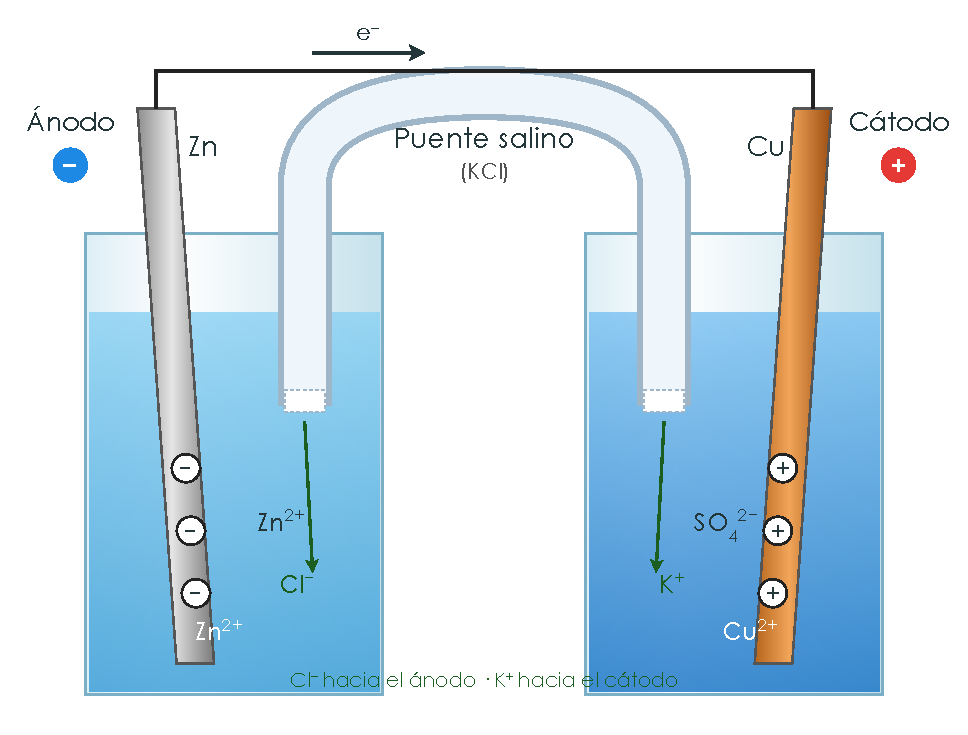
\includegraphics[width=0.6\linewidth]{FigurasSVG/UD8_Reacciones_Redox/pdf/UD8_01_puente_salino.pdf}
            \caption{Conexión del puente salino}
            \label{fig:electrodo-puente-salito}
        \end{figure}
    \end{enumerate}

    Este puente salino es fundamental para permitir el flujo de los iones entre las celdas para mantener un equilibrio de la carga eléctrica permitiendo así que la reacción redox continúe.

    En el ejemplo anterior, podemos ver como en el caso del electrodo de \ch{Zn} se irá perdiendo cargas negativas por lo que será necesario introducir más cargas negativas en forma de \ch{Cl-} o bien eliminando del sistema cargas positivas en forma de \ch{Zn\pch[2]}.
    Justamente lo contrario sucede en el caso del electrodo de cobre.
    En este caso, se irá eliminando de la disolución iones positivos por lo que tendremos que introducir más iones positivos en forma de \ch{K+} o bien eliminando carga negativa en forma de el anión que forme el electrodo de cobre.

    \subsection{Funcionamiento de una Pila}\label{subsec:funcionamiento-de-una-pila}

% \subsection{Pilas galvánicas}

    Las conocidas pilas galvánicas están basadas en reacciones entre especies en disolución acuosa y están formadas por dos electrodos comunicados eléctricamente e iónicamente.
% Esta comunicación está formado por:

% \begin{itemize}
%     \item Un \negrita{conductor sólido} para que los electrones puedan ir de un electrodo a otro, desde el más negativo al más positivo.
%     \item Un \negrita{tabique poroso} de porcelana o vidrio o un \negrita{puente salino} formado por un tubo en \(U\) taponado con algodón o lana de vidrio en los extremos y que contiene una solución conductora de una sal inerte como por ejemplo \ch{KCl} o \ch{HNO3}.
% \end{itemize}

    En el ánodo (polo negativo de la pila), se produce la oxidación, y los electrones pasan pasar a través del sólido conductor al cátodo donde se produce la reducción produciéndose así al movimiento de los electrones hasta que se iguale la carga neta y se llegue al equilibrio.
    La función del puente salino será evitar que se llegue a ese equilibrio hasta que no se hayan agotado los reactivos tal y como se comentó en el apartado anterior.

% Estos dos sistemas, permite la difusión de los iones de una disolución a otra, para igualar la carga neta, evitando así que el sistema llegue al equilibrio continuando así el proceso hasta que se produzca el agotamiento entre los reactivos.


% Una pila por tanto consiste en la separación física de dos componentes de una reacción redox, de modo que los electrones van de una sustancia que se oxida a la que se reduce a través de un circuito eléctrico. Este proceso se puede aprovechar para generar, luz, calor, trabajo \(\dots\)

% Se sabe que los electrones van del electrodo negativo al positivo pero que el sentido de la corriente se toma desde el polo positivo al negativo.

% En las pilas tendremos:

% \begin{itemize}
%     \item \negsubro{Ánodo}. Es el electrodo \negrita{negativo} y es donde se produce la \negrita{oxidación}.
%     \item \negsubro{Cátodo}. Es el electrodo \negrita{positivo} y es donde se produce la \negrita{reducción}.
% \end{itemize}

    Consideremos la Pila de Daniell formada por los electrodes de \ch{Zn} y de \ch{Cu} sumergidos en disoluciones de sus correspondientes sulfatos.
    \begin{center}
        \begin{itemize}
            \item \negsubro{Ánodo (Polo negativo)}. \(\ch{Zn - 2 \el -> Zn\pch[2]}\)
            \item \negsubro{Cátodo (Polo positivo)}. \( \ch{Cu^{2+} + 2 \el -> Cu}\)
        \end{itemize}
    \end{center}

    \begin{figure}[H]
        \centering
        % [FIGURA ORIGINAL] \includegraphics[scale=.45]{images/imagesUD8ReaccionesRedox/UD8_Teoria/pila_de_daniell}
        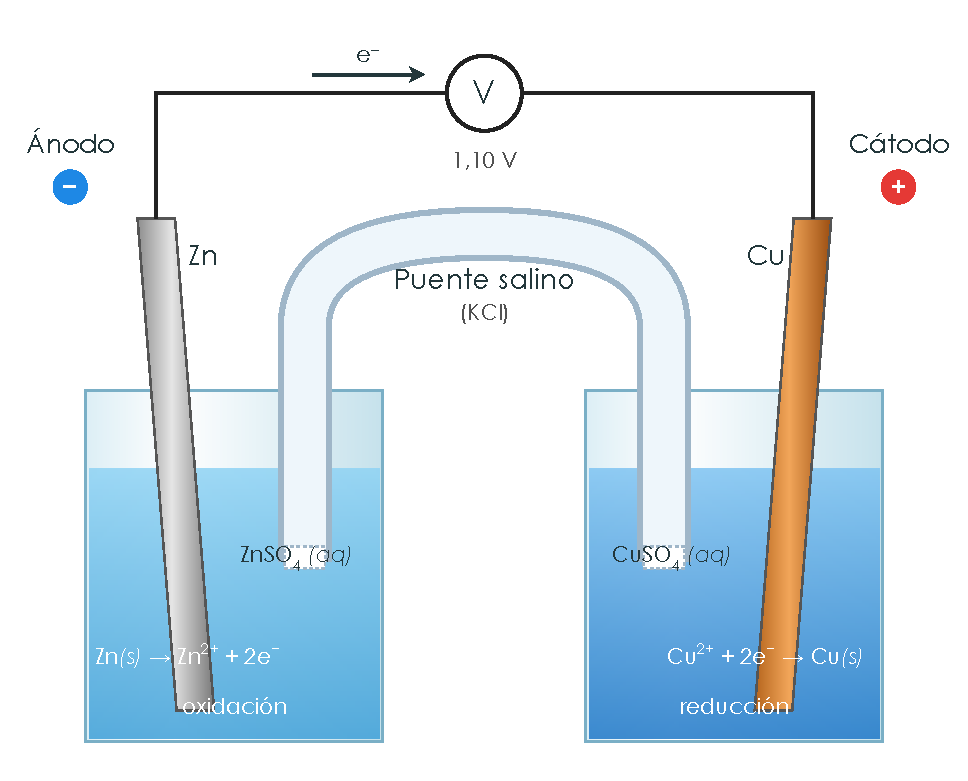
\includegraphics[width=0.65\linewidth]{FigurasSVG/UD8_Reacciones_Redox/pdf/UD8_02_pila_daniell.pdf}
        \caption{Pila de Daniell}
        \label{fig:Pila-de-Daniell}
    \end{figure}

    \subsection{Notación de una pila}\label{subsec:notacion-de-una-pila}

    Una pila se describe a partir de la notación de los electrodos pero separando ahora ambos electrodos con una doble barra \(||\).

    Por convenio, se escribe la reacción que tiene lugar en el ánodo (oxidación) a la izquierda y la reacción que tiene lugar en el cátodo (reducción) a la derecha.
    Para un electrodo formado por los electrodos vistos anteriormente tendríamos que:
    \begin{equation*}
        \underbrace{\ch{(Pt)\  Fe\pch[2]}\ |\ \ch{Fe\pch[3]} (0.05 \si{\M})}_{\text{\rojon{Ánodo}}}  \ || \ \underbrace{\ch{Cl2} (\SI{1}{\atmospher})\ | \ \ch{2 Cl-} (0.75 \si{\M})\ \ch{(Pt)}}_{\text{\azuln{Cátodo}}}
    \end{equation*}


% \begin{equation*}
%     \eqnmarkbox[blue]{node1}{m} = \eqnmarkbox[red]{node2}{\text{E}_q}\cdot \eqnmarkbox[orange]{node3}{I} \cdot \eqnmarkbox[green]{node4}{t}
% \end{equation*}
% \annotate[yshift=1em]{left}{node1}{masa depositada en (g)}
% \annotate[yshift=1em]{}{node2}{equivalente electroquímico (g/C)}
% \annotate[yshift=-1em]{below,left}{node3}{Intensidad de corriente (A)}
% \annotate[yshift=1em]{below}{node4}{tiempo (s)}

    \subsection{Potenciales del electrodo y de la pila}\label{subsec:potenciales-del-electrodo-y-de-la-pila}

    La diferencia de potencial entre los electrodos y la disolución con la que están en contacto se denomina \negrita{potencial de contacto} o \negrita{potencial eléctrico}.
%  y es imposible medirlo ya que no se puede conectar la disolución a un instrumento de medida. La única manera de medirlo es introduciendo en ella un nuevo electrodo denominado \negrita{electrodo de referencia}.

    \begin{center}
        \begin{definicion}[width=0.9\textwidth]{Fuerza Electromotriz}
            Llamamos \negrita{fuerza elctromotriz (fem)} de una pila como la diferencia de potencial entre sus electrodos
        \end{definicion}
    \end{center}


    Esta diferencia de potencial la podemos medir con un voltímetro y se definir como el potencial de reducción del cátodo menos el potencial de reducción del ánodo:

    \begin{gather*}
        \varepsilon_{\text{pila}} = \varepsilon_{\text{red cátodo}} - \varepsilon_{\text{red ánodo} } \separ
        \varepsilon_{\text{pila}}  = \varepsilon_+ - \varepsilon_-
    \end{gather*}


% \subsection{Potenciales normales de reducción}

% Cuando tenemos dos electrodos algunas veces nos enfrentamos a la cuestión ¿cuál de los dos electrodos actúa como ánodo y cuál como cátodo? para resolver esta cuestión nos tenemos que fijar los los potenciales normales de reducción de los diferentes electrodos, es decir al potencial creado por cada electrodo cuando se ha conectado a un electrodo de referencia para medirlo (este electrodo de referencia es el de hidrógeno al que se le asigna el valor de \SI{0}{\volt}).

% Al final del tema, tenéis una tabla con los principales potenciales de reducción de las distintas especies.

% \caja{Definimos \negrita{potencial normal o estándar} de un electrodo al potencial calculado a \temperatura[c]{25} de temperatura, a concentración \SI{1}{\M} de las especies en disolución y a la presión de \SI{1}{\bar} si en él interviene gases}



    \caja{Las especies con mayores potenciales de reducción tendrán más tendencia a reducirse actuando como oxidantes}

    Mientras que:

    \caja{Las especies con menores potenciales de reducción tenderán a oxidarse actuando en este caso como reductores}

    Para determinar las especies que se reducen (están en el cátodo) y las especies que se oxidan (en el ánodo) debemos fijarnos en los correspondientes potenciales normales o estándar de reducción.
    La especie con mayor potencial, mayor tendencia a reducirse (estará en el cátodo) mientras que la especie con menor potencial de reducción tendrá menos tendencia a reducirse (más tendencia a oxidarse)

    \subsection{Electrodo de hidrógeno}\label{subsec:electrodo-de-hidrogeno}

    Está constituido por una disolución de hidrones de concentración \concentracion[m]{1}, a través de la cual, se burbujea \ch{H2} a la presión de \SI{1}{\bar}.
    Una varilla de platino sirve para establecer el contacto eléctrico.
    La reacción que tiene lugar en el electrodo es:
    \begin{equation*}
        \ch{2 H+ \aq{} + 2 \el -> H \gas{}}
    \end{equation*}

    Siendo la notación, por tanto, de dicho electrodo como:

    \begin{equation*}
        \ch{(Pt)\ 2 H+ } \ (\SI{1}{\m})\ | \ \ch{H2 \gas}
    \end{equation*}

    \subsection{Trabajo o energía de una pila}\label{subsec:trabajo-o-energia-de-una-pila}

    Al ser la pila un sistema termodinámico realizará por tanto un trabajo eléctrico que consiste en transportar la carga eléctrica desde el ánodo al cátodo siendo este trabajo la multiplicación entre la carga transportada \(Q\) y la \(fem\).

    \begin{equation*}
        W = -Q\ \varepsilon
    \end{equation*}

    Esta carga \(Q\) la podemos tomar como \(Q = n\ F\) siendo \(n\) el \negrita{número de moles de electrones} transportados y \(F\) la constante de Faraday que establece la carga por mol de electrones, siendo su aproximado de \(F = \SI{96500}{\coulomb\per\mol}\)

    La expresión anterior del trabajo la podemos escribir como:

    \begin{equation}
        W = -n\ F\ \varepsilon
        \label{eq:trabajo-fuerza-electromotriz}
    \end{equation}

    En todo proceso termodinámico que se lleve a cabo a presión y temperatura constante, se cumple que \(\Delta G  = W_{\text{rev}} \).
    Por lo tanto en el caso de la pila tendremos que:

    \begin{equation}
        \Delta G = -n\ F\ \varepsilon
        \label{eq:energia-libre-giibs-fuerza-electromotriz}
    \end{equation}

    O en condiciones estándar

    \begin{equation}
        \Delta G\text{º} = -n\ F\ \varepsilon\text{º}\label{eq:G-vs-faraday}
    \end{equation}

    Analizando la \(fem\) tendremos que:

    \begin{itemize}
        \item Si \(\varepsilon_{\text{pila}} > 0\), entonces la reacción será \negrita{espontánea} debido a que \(\Delta G <0\).
        \item Si \(\varepsilon_{\text{pila}} < 0\), entonces la reacción \negrita{no} será \negrita{espontánea} debido a que \(\Delta G > 0\).
        \item Si \(\varepsilon_{\text{pila}} = 0\), la reacción estará en equilibrio debido a que \(\Delta G = 0\).
    \end{itemize}

%    \subsection{Relación entre el potencial redox y la concentración. Ecuación de Nerst}
%
%    La ecuación de Nerst relaciona el potencial de la la pila o los electrodos con la concentración de dichas especies, ya que el potencial irá cambiando según la concentración de dichas especies. La ecuación de Nerst es la siguiente:
%
%    \begin{equation}
%        \tcboxmath[opteqA]{\varepsilon = \varepsilon\text{º} - \dfrac{R\ T}{n\ F}\ \ln k}
%    \end{equation}
%
%    siendo \(k\) la constante de equilibrio referida a las concentraciones
%
%    Tradicionalmente la ecuación de Nerst se ha expresado en función de logaritmos decimales en lugar de logaritmos neperianos por lo que si hacemos un cambio de base en el logaritmo y operamos la constante de los gasees y la constante de Faraday tendremos que:
%
%    \begin{equation}
%        \tcboxmath[opteqA]{\varepsilon = \varepsilon\text{º} - \dfrac{0.059}{n}\ \ln k}
%    \end{equation}
%
%    \subsubsection{Potencial de un electrodo}
%
%    Sea la reacción general del electrodo:
%
%    \begin{equation*}
%        \text{Forma oxidada} + n\ \el -> \text{Forma reducida}
%    \end{equation*}
%
%    La ecuación de Nerst adopta la forma de:
%
%    \begin{equation*}
%        \varepsilon = \varepsilon\text{º} - \dfrac{R\ T}{n\ F}\ \ln \dfrac{\conc{Redudica}}{\conc{Oxidada}}
%    \end{equation*}
%
%    \subsubsection{Potencial de una pila}
%
%    Ya hemos visto anteriormente que el potencial de una pila, será el potencial del cátodo menos el potencial del ánodo (\(\varepsilon_{\text{pila}} = \varepsilon_+ - \varepsilon_-\) )
%
%    Por lo tanto, el potencial de reducción de la pila (\(\varepsilon_{\text{pila}}\)) debe cumplir la ecuación de Nerst aplicada a la ecuación completa de la reacción química. Consideremos la reacción química general:
%
%    \begin{equation*}
%        \ch{a\ Oxidante_1 + b\ Reductor_2 -> m\ Reductor_1 + n\ Oxidante_2}
%    \end{equation*}
%
%    El potencial por tanto de la pila sería:
%
%    \begin{gather*}
%        \varepsilon_{\text{pila}} = \varepsilon\text{º} - \dfrac{R\ T}{n\ F}\ \ln \dfrac{\conc{Reductor_1}^m\ \conc{Oxidante_2}^n}{\conc{Reductor_2}^b\ \conc{Oxidante_1}^a}
%    \end{gather*}
%
%    Tal y como se vió anteriormente, en la constante de equilibrio solo se indican las especies en disolución o en estado gaseoso, así por ejemplo la ecuación de Nerst para la pila de Daniell quedaría según:
%
%    \begin{equation*}
%        \ch{Zn\sld{} + Cu\pch[2]\aq{} <=> Zn\pch[2]\aq{} + Cu\sld{}}
%    \end{equation*}
%
%    \begin{equation*}
%        \varepsilon_{\text{pila}} = \varepsilon\text{º} - \dfrac{R\ T}{n\ F}\ \ln \dfrac{\conc{Zn\pch[2]}}{\conc{Cu\pch[2]}}
%    \end{equation*}

%? \section{Aplicaciones electroquímicas} no poner esta sección.

%? \section{Corrosión de metales} no poner esta sección.


    \section{Electrolisis}\label{sec:electrolisis}

    \begin{center}
        \begin{definicion}[width=0.9\textwidth]{Electrolisis}
            La \negrita{electrolisis} consiste en una reacción química desencadenada por el paso de corriente eléctrica a través de un electrolito o disolución conductora de la electricidad
        \end{definicion}
    \end{center}


% Por ejemplo, el proceso que tiene lugar en la pila de Daniell (ver ecuaciones más arriba) es espontáneo debido a que \(\varepsilon_{\text{pila}} = \varepsilon_+ - \varepsilon_- = 0.34 - (-0.76) = \SI{1.10}{\volt}\). En la pila de Daniell, el \ch{Zn} actúa como ánodo y el \ch{Cu} como cátodo.

% Si consideramos ahora el proceso inverso, es decir:

% \begin{itemize}
%     \item \negsubro{Ánodo} (electrodo / polo negativo). \(\ch{Cu - 2 \el -> Cu\pch[2]}\quad \varepsilon_- = \SI{0.346}{\volt}  \)
%     \item \negsubro{Cátodo} (electrodo / polo positivo). \( \ch{Zn^{2+} + 2 \el -> Zn}\quad \varepsilon_+ = \SI{-0.7628}{\volt} \)
% \end{itemize}

% Si analizamos el potencial de la de la pila vemos que \(\varepsilon_{\text{pila}} = \varepsilon_+ - \varepsilon_- = -0.76 - (0.346) = \SI{-1.106}{\volt}\) vemos que \(\varepsilon_{\text{pila}}<0\) y por tanto la reacción no será espontánea. Si establecemos una diferencia de potencial superior a \SI{1.10}{\volt} tendría lugar la reacción utilizando al \ch{Zn} como polo cátodo (polo positivo) y al \ch{Cu} como ánodo (polo negativo)

% Al sistema de estos dos electrodos más la fuente de potencial externa se le conoce como \negrita celda electrolítica. Y en este caso los electrodos serán:

    La electrolisis tiene muchas aplicaciones como la producción de metales así como la producción de no metales como el cloro y el fluor.

    Para realizar una electrolisis necesitamos:

    \begin{itemize}
        [label={\color{myOrange3} \(\blacksquare\)}]
        \item \negsubro{Fuente de corriente continua}.
        Proporciona la corriente eléctrica y tiene que ser continua y con un voltaje lo suficiente para que se produzca la reacción.
        Esta fuente está unidad a los electrodos mediante un hilo conductor.
        Este generador ni crea ni destruye electrones, tan solo los aporta al polo negativo y los absorbe por el polo positivo.
        \item Un \negsubro{electrodo negativo} denominado \negrita{cátodo} es donde se produce la reducción.
        \item Un \negsubro{electrodo positivo} denominado \negrita{ánodo} es donde se produce la oxidación.
        \item \negsubro{Cuba o celda electrolítica}.
        Es donde se contiene la disolución o el electrolito fundido donde se sumergen los electrodos.
    \end{itemize}

    Un error común es asignar al ánodo el polo negativo siempre y al cátodo el polo positivo, pero como vemos ahora el proceso es a la inversa.
    En realidad ánodo hace referencia al polo por el cual salen los electrones y cátodo al polo por donde entran los electrones.

    Cuando establezcamos las correspondientes reacciones que suceden en una electrolisis con sus correspondientes potenciales, veremos que el potencial final de la reacción será negativo.
    Este potencial nos indicará qué potencial externo debemos administrar para que se produzca la electrolisis.

    \subsection{Electrolisis del agua}\label{subsec:electrolisis-del-agua}

    \negsubro{NOTA IMPORTANTE:} los potenciales que se pondrán en las siguientes reacciones serán los correspondientes a dicha reacción y no deben tomarse como potenciales de reducción.
    Para calcular el potencial de sistema tendremos que sumar ambos potenciales.

    Si introducimos dos electrodos en una celda electrolítica y aplicamos una diferencia de potencial de \SI{2.06}{\volt} el agua se descompondrá en hidrógeno y en oxígeno tal y como se muestran en las siguientes reacciones.

    \begin{equation*}
        \begin{array}{rrcll}
        {\color{blue} \text{Cátodo}\ (-)\ \text{Reducción}}
            : & \ch{2 H2O + 2 \el{}} & \ch{->} & \ch{ H2 + 2 OH-}    & \varepsilon\text{º} = \SI{-0.83}{\volt}                \separ
            {\color{blue}\text{Ánodo}\ (+)\ \text{Oxidación}}:   & \ch{2 H2O}        & \ch{->} & \ch{O2 + 4 H+ + 4 \el}   & \varepsilon\text{º} = \SI{-1.23}{\volt} \separ
            \midrule
            {\color{blue} \text{Reacción global} }:              & \ch{2 H2O\lqd{}}    & \ch{->} & \ch{2 H2\gas{} + O2\gas{}}  & \varepsilon\text{º}_\text{reacción} = \SI{-2.06}{\volt}
        \end{array}
    \end{equation*}

    En este caso, tendríamos que aplicar un potencial dé al menos \SI{2.06}{\volt} para llevar a cabo la hidrólisis.

% \begin{equation*}
%     \begin{array}{rrcl}
%         {\color{blue} \text{Cátodo}\ (-)\ \text{Reducción}}: & \ch{2 H+ + 2 \el} & \ch{->} & \ch{2 H2}                      \separ
%         {\color{blue}\text{Ánodo}\ (+)\ \text{Oxidación}}:   & \ch{2 H2O}        & \ch{->} & \ch{O2 + 4 H+ + 4 \el}    \separ
%         \midrule
%         {\color{blue} \text{Reacción global} }:              & \ch{2 H2O\lqd{}}    & \ch{->} & \ch{2 H2\gas{} + O2\gas{}} 
%     \end{array}
% \end{equation*}

    \subsubsection{Técnicas de electrolisis del agua}

    Estas técnicas varían en función de la cantidad de \ch{H2} y de \ch{O2} que se quiera generar.

    \negsubro{Electrolisis con agua ácida}

    Si la reacción de electrolisis se realiza en medio ácido, las reacciones que tendríamos serían:

    \begin{equation*}
        \begin{array}{rrcll}
        {\color{blue} \text{Cátodo}\ (-)\ \text{Reducción}}
            : & \ch{2 H+ + 2 \el{}} & \ch{->} & \ch{  H2 }    & \varepsilon\text{º} = \SI{0.00}{\volt}                \separ
            {\color{blue}\text{Ánodo}\ (+)\ \text{Oxidación}}:   & \ch{2 H2O }        & \ch{->} & \ch{ O2 + 4 H+ + 4 \el{}}   & \varepsilon\text{º} = \SI{-1.23}{\volt} \separ
            \midrule
            {\color{blue} \text{Reacción global} }:              & \ch{2 H2O\lqd{}}    & \ch{->} & \ch{2 H2\gas{} + O2\gas{}}  & \varepsilon\text{º}_\text{reacción} = \SI{-1.23}{\volt}
        \end{array}
    \end{equation*}

    En este caso, tendríamos que aplicar un potencial dé al menos \SI{1.23}{\volt} para llevar a cabo la hidrólisis.

    \negsubro{Electrolisis con agua alcalina}

    La electrolisis también se puede llevar a cabo con soluciones básicas como \ch{KOH} o \ch{NaOH}.
    En este caso, las reacciones que tendrían lugar serían:

    \begin{equation*}
        \begin{array}{rrcll}
        {\color{blue} \text{Cátodo}\ (-)\ \text{Reducción}}
            : & \ch{2 H2O + 2 \el{}} & \ch{->} & \ch{ H2 + 2 OH-}    & \varepsilon\text{º} = \SI{-0.83}{\volt}                \separ
            {\color{blue}\text{Ánodo}\ (+)\ \text{Oxidación}}:   & \ch{2 OH- }        & \ch{->} & \ch{2 O2 + 2 H2O + 4 \el{}}   & \varepsilon\text{º} = \SI{-0.41}{\volt} \separ
            \midrule
            {\color{blue} \text{Reacción global} }:              & \ch{2 H2O\lqd{}}    & \ch{->} & \ch{2 H2\gas{} + O2\gas{}}  & \varepsilon\text{º}_\text{reacción} = \SI{-1.24}{\volt}
        \end{array}
    \end{equation*}




    \subsection{Electrolisis de una sal fundida}\label{subsec:electrolisis-de-una-sal-fundida}

    Si tenemos una sal como el \ch{NaCl} fundida, al sumergir los electrodos y conectar la corriente continua, los iones \ch{Cl-} se oxidan en el ánodo, descargándose según la reacción siguiente:

    \begin{equation*}
        \begin{array}{rrcll}
        {\color{blue} \text{Cátodo}\ (-)\ \text{Reducción}}
            : & \ch{ Na+ + 1 \el{}} & \ch{->} & \ch{Na}  & \varepsilon\text{º} = \SI{-2.71}{\volt}                 \separ
            {\color{blue}\text{Ánodo}\ (+)\ \text{Oxidación}}:   & \ch{2 Cl-}        & \ch{->} & \ch{Cl2 + 2 \el{}}  & \varepsilon\text{º} = \SI{-1.36}{\volt}  \separ
            \midrule
            {\color{blue} \text{Reacción global} }:              & \ch{2 NaCl}    & \ch{->} & \ch{2 Na + Cl2} & \varepsilon\text{º}\subin{reacción} = \SI{-4.07}{\volt}
        \end{array}
    \end{equation*}

    Otro ejemplo sería el de la sal de  \ch{CuCl2}, en este caso analizando los potenciales normales de reducción de ambas especies, en el ánodo se desprenderá \ch{Cl2}  en el cátodo se recubrirá de una película brillante de \ch{Cu}.
    La reacciones que tienen lugar son:

    \begin{equation*}
        \begin{array}{rrcll}
        {\color{blue} \text{Cátodo}\ (-)\ \text{Reducción}}
            : & \ch{Cu\pch[2] + 2 \el} & \ch{->} & \ch{Cu}                   & \varepsilon\text{º} = \SI{0.346}{\volt} \separ
            {\color{blue}\text{Ánodo}\ (+)\ \text{Oxidación}}:   & \ch{2 Cl-}             & \ch{->} & \ch{Cl2 + 2 \el}          & \varepsilon\text{º} = \SI{1.359}{\volt} \separ
            \midrule
            {\color{blue} \text{Reacción global} }:              & \ch{CuCl2\aq{}}        & \ch{->} & \ch{Cu\sld{} + Cl2\gas{}} & \varepsilon\text{º}_{\text{reacción}} = \SI{-1.013}{\volt}
        \end{array}
    \end{equation*}

    \subsection{Electrolisis de una sal disuelta}\label{subsec:electrolisis-de-una-sal-disuelta}

    Si realizamos la electrolisis con sales disueltas en disolución acuosa, el agua presente en la disolución compite con los iones provenientes de la sal y la electrolisis sufre algunas modificaciones.

    Como ejemplo, estudiaremos la electrolisis de una disolución acuosa de \ch{NaCl}.

    En este caso tendremos dos posibles reacciones de oxidación y debemos determinar cuál de ellas es la que se produce:

    \begin{equation*}
        \begin{array}{rcll}
            \ch{2 H2O } & \ch{->} & \ch{O2 + 4 H+ + 4 \el{}}  & \varepsilon\text{º} = \SI{-1.23}{\volt}   \separ
            \ch{2 Cl-}        & \ch{->} & \ch{Cl2 + 2 \el{}}  & \varepsilon\text{º} = \SI{-1.36}{\volt}
        \end{array}
    \end{equation*}



    Debido a que en un disolución de una sal además de la correspondiente sal tenemos \water{} esta puede competir en la reacción de hidrólisis y por tanto hay que analizar los correspondientes potenciales normales de reducción.
    Así por ejemplo en el caso de la hidrólisis de una disolución acuosa de \ch{NaCl}, las reacciones que tienen lugar son:

    \begin{equation*}
        \begin{array}{rrcll}
        {\color{blue} \text{Cátodo}\ (-)\ \text{Reducción}}
            : & \ch{2 H+ + 2 \el{}}& \ch{->} & \ch{ H2} & \varepsilon\text{º} = \SI{0}{\volt} \separ
            {\color{blue}\text{Ánodo}\ (+)\ \text{Oxidación}}: & \ch{2 Cl-}& \ch{->} & \ch{Cl2 + 2 \el} & \varepsilon\text{º} = \SI{1.359}{\volt} \separ
            \midrule
            {\color{blue} \text{Reacción global} }: & \ch{2 H+ \aq{} + 2 Cl- \aq{}} & \ch{->} & \ch{H2\gas{} + Cl2\gas{}} & \varepsilon\text{º}_{\text{reacción}} = \SI{-1.359}{\volt}
        \end{array}
    \end{equation*}

    Como vemos, ahora en el cátodo, se produce la reducción de los iones  \ch{H+} en lugar de producirse la reducción del \ch{Na+} a \ch{Na} según la reacción:

    \begin{equation*}
        \ch{Na+ \aq{} + \el -> Na\sld{}}
    \end{equation*}

    Esto es debido a que el potencial normal de reducción del sodio (\(\varepsilon\text{º} = \SI{-2.71}{\volt}\)) es menor que el del hidrógeno  (\(\varepsilon\text{º} = \SI{0}{\volt}\)). Esto demuestra que los iones \ch{H+} tienen una mayor apetencia por los electrones que los iones \ch{Na+} y, por tanto, se reducen los iones  \ch{H+} y no los iones \ch{Na+}.

    De manera general podemos decir que:

    \begin{itemize}
        \item En el cátodo que es donde se producirá la reducción.
        Los cationes de mayor potencial normal de reducción serán los primeros en descargarse.
        \item En el ánodo que es donde se producirá la oxidación, los iones negativos de menor potencial de ionización serán los primeros en descargarse.
    \end{itemize}


    \section{Leyes de Faraday}\label{sec:leyes-de-faraday}

    \negrita{Michael Faraday} formuló las leyes fundamentales de la electrolisis.

    \caja{La cantidad de sustancia que sufre oxidación o redución en cada electrodo durante una electrolisis es directamente proporcional a la cantidad de electricidad que pasa a través de la disolución.}

    \begin{enumerate}[label=\numberballmDarkTeal]
        \item \negsubro{Primera ley de Faraday}.
        Las \negrita{masas} de las sustancias depositadas o liberadas en cada electrodo durante una electrolisis son proporcionales a la \negrita{cantidad de electricidad} que ha pasado a través de la celda electrolítica.
        \item \negsubro{Segunda ley de Faraday}.
        Para una misma cantidad de carga eléctrica, la masa de las sustancias depositadas o liberadas en los electrodos es proporcional a su masa atómica y al número de electrones intercambiados por cada una de ellas según la expresión:

        \begin{gather}
            Q = z\ \dfrac{m}{M_a}\cdot F  \notag \separ
            m(g) = \dfrac{M_a}{z\cdot F}\cdot Q
        \end{gather}

        \begin{itemize}
            \item \(Q\) = carga que circula en culombios.
            \item \(z\) = número de electrones intercambiados.
            \item \(m\) = masa depositada o liberada en gramos.
            \item \(M_a\) = masa atómica.
            \item \(F\) = constante de Faraday
        \end{itemize}

        Hay que tener en cuenta que:

        \begin{itemize}
            \item \textbf{Carga eléctrica(\(\bm{Q}\))}: es la carga que circula por la cuba electrolítica, y se puede expresar en función de la intensidad de corriente eléctrica, según la expresión.
            \begin{equation*}
                Q = I\cdot t
            \end{equation*}
            \item \textbf{Número de electrones (\(\bm{z}\))}: es la cantidad de electrones (mol) que necesita una sustancia para oxidarse o reducirse en un electrodo.

            Para semirreacción: \ch{Ag+ \aq{} + 1 \el{} -> Ag \sld{}} \(\Rightarrow z = 1\).

            Para la semirreacción: \ch{Cl- \aq{}  -> Cl2 \gas{} + 2 \el{}} \(\Rightarrow z = 2\).
        \end{itemize}

    \end{enumerate}


% El significado de ambas leyes se puede resumir en la siguiente ecuación:

% \vspace*{8pt}
% \begin{equation*}
%     \eqnmarkbox[blue]{node1}{m} = \eqnmarkbox[red]{node2}{\text{E}_q}\cdot \eqnmarkbox[orange]{node3}{I} \cdot \eqnmarkbox[green]{node4}{t}
% \end{equation*}
% \annotate[yshift=1em]{left}{node1}{masa depositada en (g)}
% \annotate[yshift=1em]{}{node2}{equivalente electroquímico (g/C)}
% \annotate[yshift=-1em]{below,left}{node3}{Intensidad de corriente (A)}
% \annotate[yshift=1em]{below}{node4}{tiempo (s)}
% \vspace*{8pt}

% La constante \(E_q\) o \negrita{equivalente químico} es típica de cada sustancia y representa la masa liberada por el paso de \carga[c]{1} de electricidad.

% Sabemos que \negrita{equivalente-gramo} de una sustancia es  la masa depositada por el paso de \moles{1} de electrones.

% La cantidad de electricidad que corresponde a \moles{1} de electrones se denomina \negrita{faraday} y equivale aproximadamente a \SI{96500}{\coulomb\per\mole}

